\begin{consigna}{red}
	Armar el AoN a partir del WBS definido en la etapa anterior.

	Una herramienta simple para desarrollar los diagramas es el Draw.io
	(\url{https://app.diagrams.net/}). \href{https://app.diagrams.net}{Draw.io}

	\begin{figure}[htpb]
		\centering
		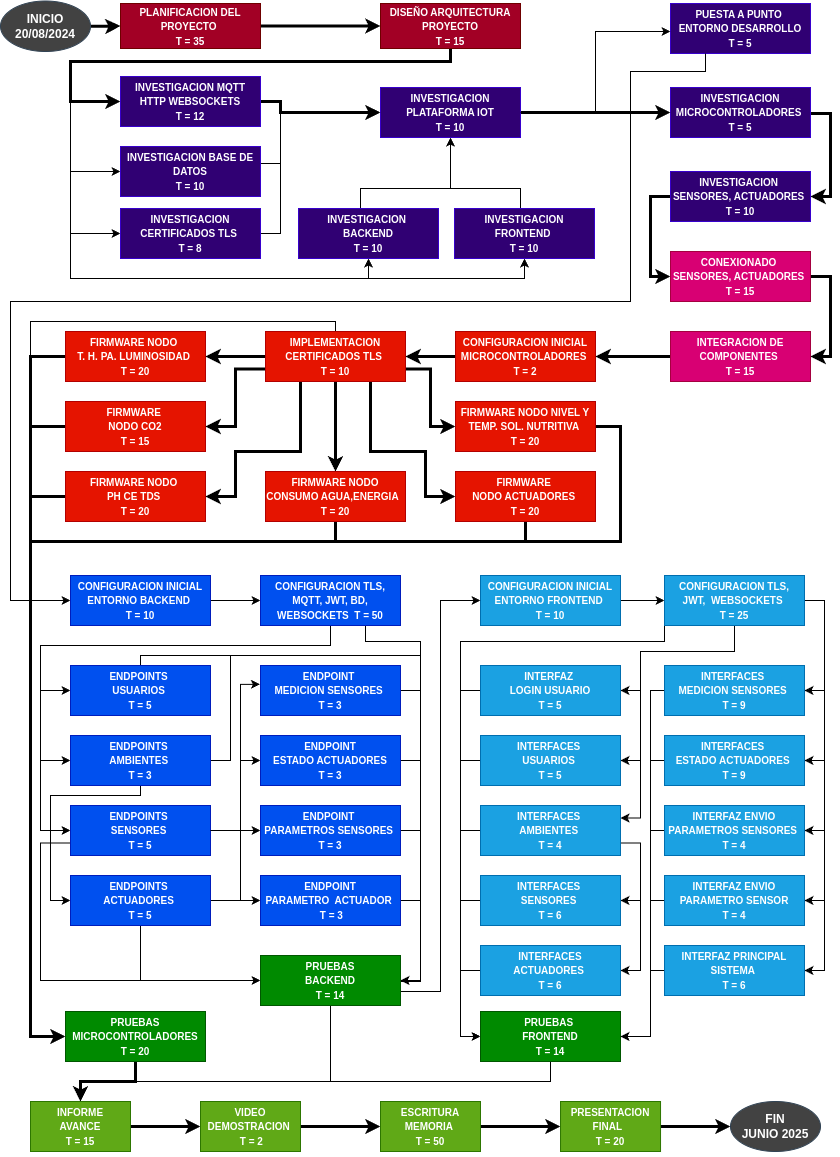
\includegraphics[width=.8\textwidth]{./Figuras/AoN.png}
		\caption{Diagrama de \textit{Activity on Node}.}
		\label{fig:AoN}
	\end{figure}

	Indicar claramente en qué unidades están expresados los tiempos. De ser
	necesario indicar los caminos semi críticos y analizar sus tiempos mediante un
	cuadro. Es recomendable usar colores y un cuadro indicativo describiendo qué
	representa cada color.

\end{consigna}